\documentclass[12pt,prb,aps,epsf]{report}
\usepackage[utf8]{inputenc}
\usepackage{amsmath}
\usepackage{amsfonts}
\usepackage{amssymb}
\usepackage{graphicx} 
\usepackage{latexsym} 
\usepackage[toc,page]{appendix}
\usepackage{listings}
\usepackage{xcolor}
\usepackage{soul}
\usepackage[T1]{fontenc}
\usepackage{amsthm}
\usepackage{mathtools}
\usepackage{setspace}
\usepackage{array,multirow,makecell}
\usepackage{geometry}
\usepackage{textcomp}
\usepackage{float}
%\usepackage{siunitx}
\usepackage{cancel}
%\usepackage{tikz}
%\usetikzlibrary{calc, shapes, backgrounds, arrows, decorations.pathmorphing, positioning, fit, petri, tikzmark}
\usepackage{here}
\usepackage{titlesec}
%\usepackage{bm}
\usepackage{bbold}

\geometry{hmargin=2cm,vmargin=2cm}

\begin{document}
	
	\title{MP 07 Instruments d'optique}
	\author{Hugo}
	
	\maketitle
	
	\tableofcontents
	
	\pagebreak
	
	
\section{Introduction}
Omniprésence des systèmes optiques : donner des exemples.\\
Donner le déroulement et l'intéret de ce montage.	

\section{Modèle de microscope}
Description du montage, liste de matériel, et intérêt du dispositif.\\

L'objectif grossit l'image de l'objet que l'on souhaite observer. L'oculaire envoi cette image à l'infini, pour que l'œil puisse l'observer sans effort.
\begin{figure}
	\centerline{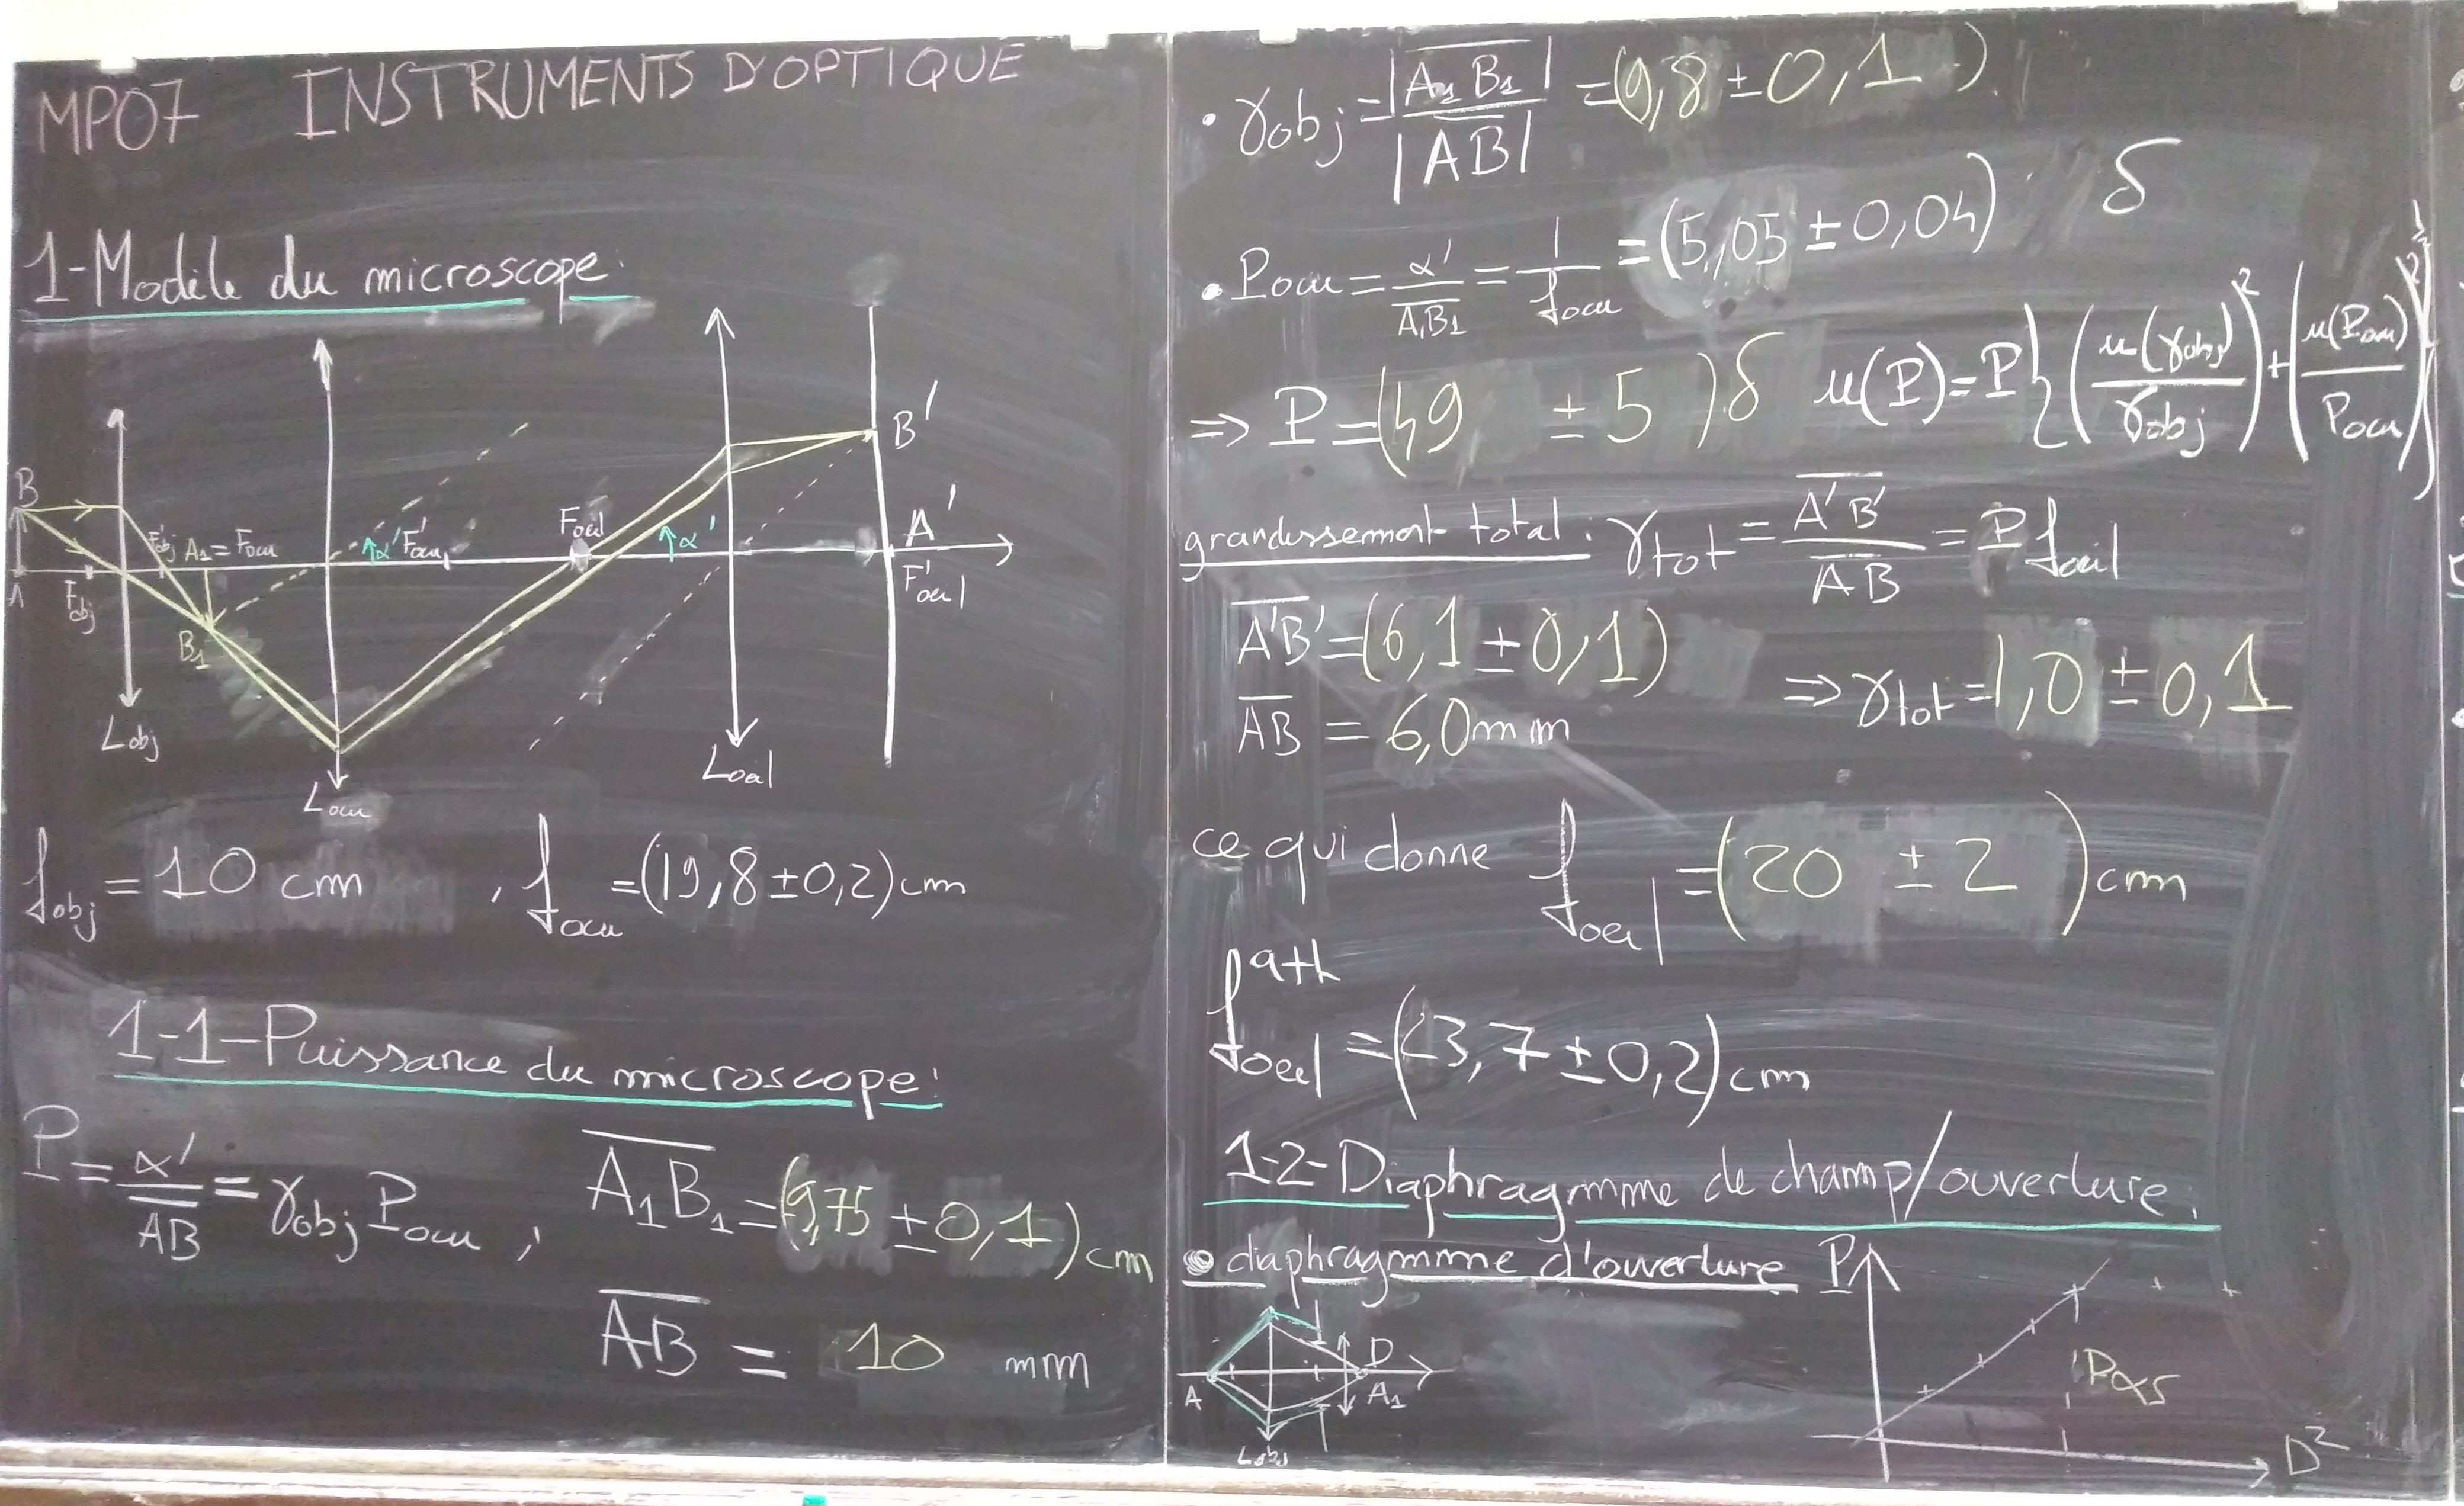
\includegraphics[width=17cm]{T1}}
\end{figure}

\subsection{Puissance du microscope}

Produit des puissances de l'objectif et de l'oculaire.
\begin{eqnarray}
P = \frac{\alpha'}{AB} = \gamma_{obj}P_{oculaire}\\
\gamma_{obj} = \frac{|A_1B_1|}{|AB|} = 9.8 +-0.1\\
P_{ocu} = \frac{\alpha'}{A_1B_1} = \frac{1}{f_{ocu}}=(5.05+-0.04) \delta\\
\Rightarrow P = 49 +- 5 \delta\\
\mathrm{avec}\; u(P) = P\left[\left(\frac{u(\gamma_{obj})}{\gamma_{obj}}\right)^2+\left(\frac{u(P_{ocu})}{P_{ocu}}\right)^2\right]
\end{eqnarray}
Grandissement total $\gamma_{tot} = \frac{A'B'}{AB}$, on le calcule et on obtient ici $\gamma_{tot} = 1.0+-0.1$

\subsection{Diagramme de champ/ouverture}
Explication du concept + schémas
\paragraph{Diaphragme d'ouverture}
\paragraph{Diaphragme de champ}


\section{Objet réel}
\begin{figure}
	\centerline{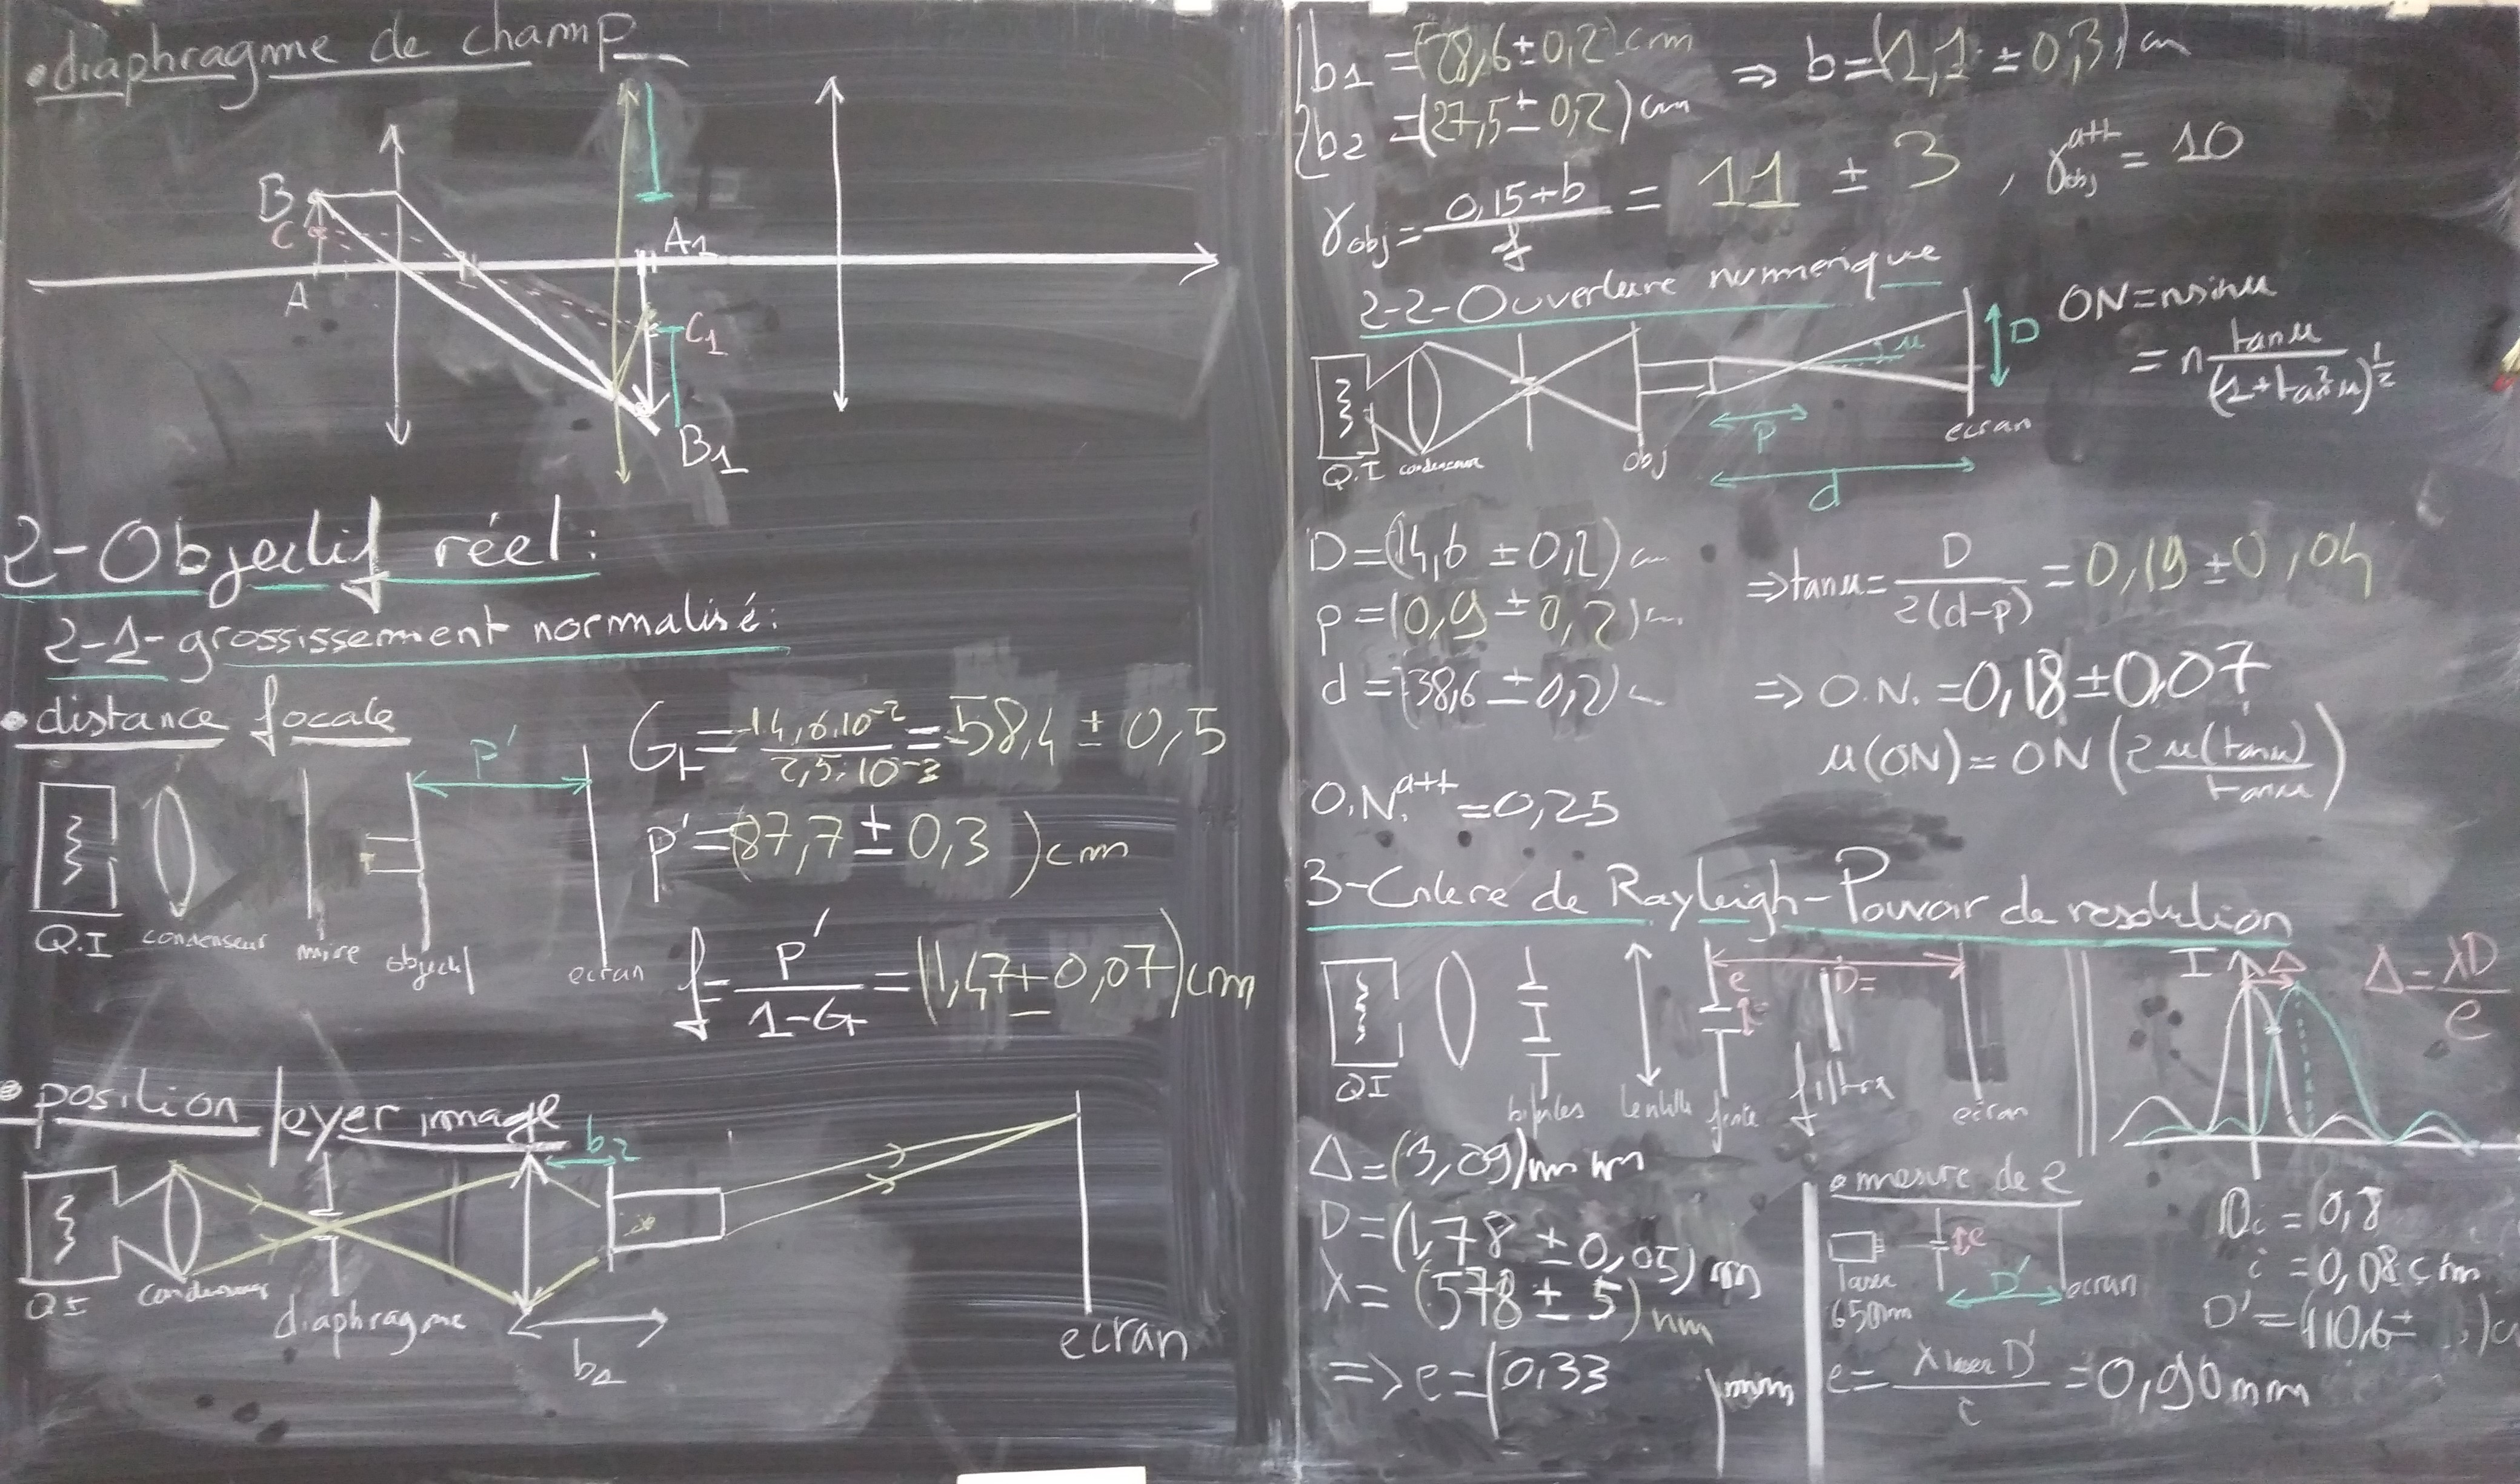
\includegraphics[width=17cm]{T2}}
\end{figure}
\subsection{Grossissement normalisé}
\paragraph{Distance focale}
On mesure ici $G-t$, $p'$ et on en déduit la focale 
\begin{eqnarray}
f = \frac{p'}{1-G_t} 
\end{eqnarray}
\paragraph{Position du foyer image}
Schéma\\
On mesure $b_1$ et $b_2$, et on en déduit $b$

\subsection{Ouverture numérique}
Définit la quantité de lumière qui rentre dans l'objectif.
\begin{eqnarray}
ON = \mathrm{ouverture}\; \mathrm{numérique} = n\sin(u) =  \frac{n\tan(u)}{\sqrt{1+\tan^2(u)}}
\end{eqnarray}
On mesure donc $p$, $d$ et $D$ puisque 
\begin{eqnarray}
\tan(u) = \frac{D}{2(d-p)}
\end{eqnarray}
L'ouverture numérique est un aspect essentiel du problème ici puisqu'elle détermine le pouvoir de résolution.

\subsection{Critère de Rayleigh - pouvoir de résolution}

Observation de l'image "diffractée" d'une double fente à l'aide d'une camera CCD.\\
Dans le cas d'un microscope la puissance de résolution n'est pas inversement proportionnelle à e mais à l'ON (fermeture du diaphragme donc).

\section{Questions}
Qu'entendez vous par critère de Rayleigh ? Quel est son sens ?\\

Les 2nd minimas sont dans le bruit ici, comment les faire sortir ? c.a.d quel est le rôle du philtre ici ?\\

Quel philtre utiliser et ou le placer ? Y a t'il une position plus judicieuse ?\\
Philtre laissant passer "une seule" longueur d'onde, placée devant la CCD.\\

(D'où vient le font (bruit lumineux) ?)\\

Est il possible d'envisager un autre type de filtrage ?\\

Mesure t'on p depuis la sortie de l'objectif ou depuis sa sortie (en principe) ?\\
Il faudrait connaître la position du plan principal image.\\

Qu'est ce qui explique que la focale de l'œil calculée soit si loin de la valeur attendue ?\\

..... Comment diminuer la profondeur de champ afin de d'améliorer la précision des mesures ?\\

\paragraph{Montage surprise} comment feriez vous pour mesurer la position d'une image virtuelle ?\\ c.a.d si je considère le microscope : où est l'image?


\section{Remarques}
C'est bien de mesurer les distances avec une ficelle. Toujours essayer de mesurer les plus de franges pour les intervalles (penser notamment à l'orientation de la feuille).\\
Il faut montrer que l'on prend la manip au sérieux.\\
Pas le temps : si résultat pas cohérent, il faut botter en touche.\\
Toujours énoncer les grandeurs lorsqu'on donne les résultats.\\
Ne pas donner de jugement de valeur : "l'ouverture numérique est le paramètre LE PLUS important".\\
Ne pas faire de liens logiques inexistant en plaçant des "donc".\\
Attention à l'alignement des instruments d'optiques sur le banc : attention à l'horizontalité !\\
Pour placer l'oculaire : pas au jugé, utiliser le $f_i$ donné par le constructeur.\\
Éclairer la fente source en plaçant l'image de la source par le condenseur dessus.\\
Les mesures ajoutées à une courbe en direct ont peu de chance de fiter dans ce genre de manip : faire deux courbe : une sans ajout et une avec : les tracer de 2 couleur différentes et modéliser celle avec que les mesures faites à la suite.\\

Trop long ici : maintenant en 30 min, on a pas le temps de mettre en valeur les liens entre les parties, il faut sélectionner les manip permettant de montrer que l'on sait maniper.\\
Ici garder le 1 mais enlever le diaphragme d'ouverture ou bcp raccourcir car seulement qualitatif.\\
Pour le critère de Rayleigh : ne pas faire trop grand sinon pas assez de lumière. Mais sinon manip à garder car utilise diffraction + CCD.\\
Peut être enlever la manip sur l'ON pour que ça rentre.



\end{document}